\documentclass[a4paper, 12pt]{article}
\usepackage[utf8]{inputenc}
\usepackage{geometry}
\usepackage{polski}
\usepackage{graphicx}
\usepackage{float}
\usepackage{etoolbox,refcount}
\usepackage{multicol}

\newgeometry{left=2cm, right=2cm, bottom=1.5cm, top=1.5cm}

\begin{document}
	\begin{figure}[H]
		\centering
		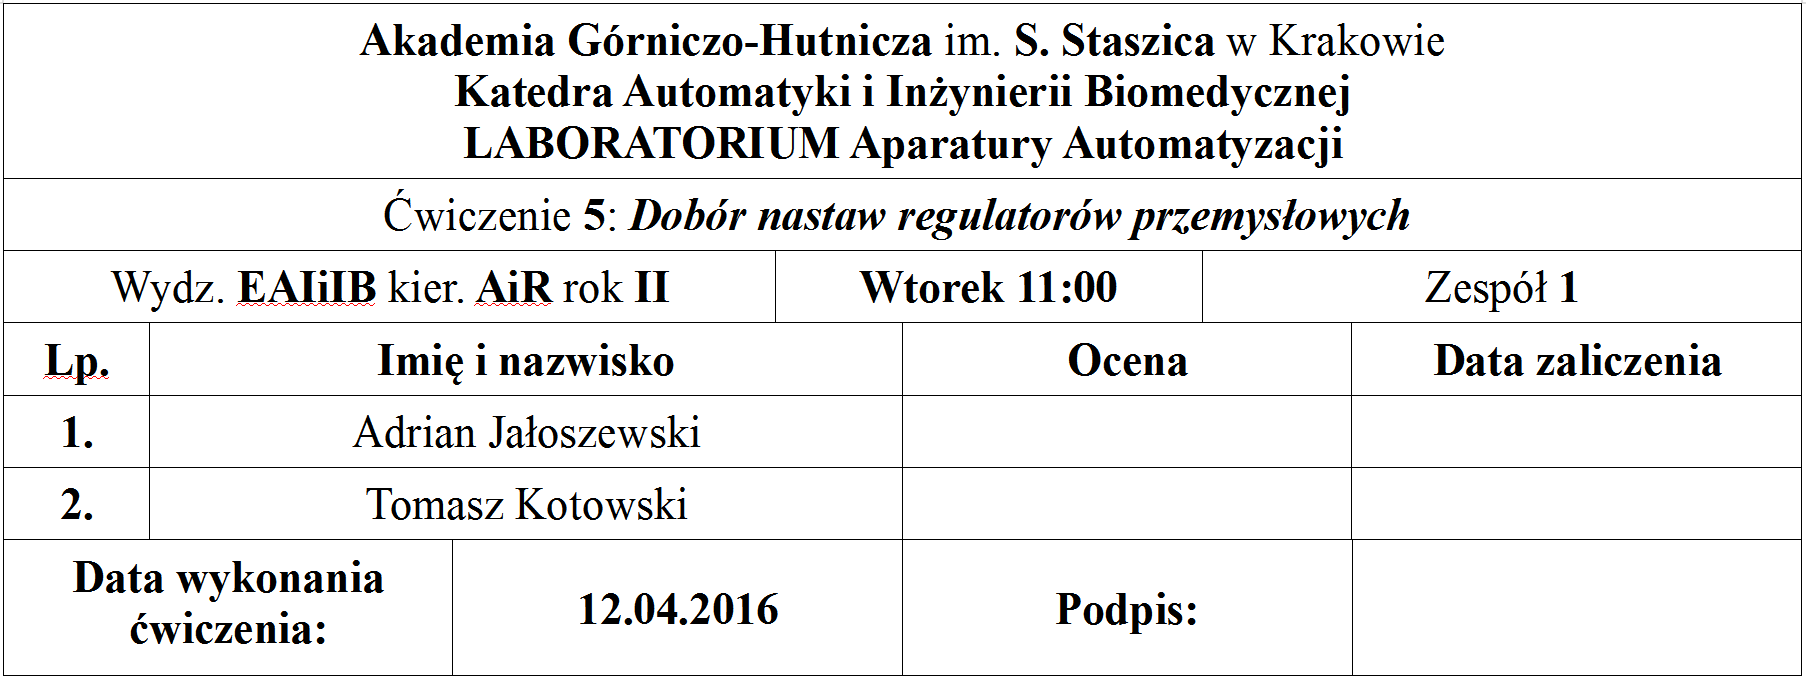
\includegraphics[height=6cm, width=\textwidth]{./img/Capture.PNG}
	\end{figure}
	\section{Cel ćwiczenia}
		Celem ćwiczenia jest zapoznanie się z metodami strojenia i samostrojenia regulatorów przemysłowych na podstawie metod: Zieglera-Niecholsa, Astroma--Hagglunda oraz Takahashi'ego jak \linebreak i zapoznanie się z praktyczną realizacją procedury samostrojenia w rzeczywistym regulatorze.
	\section{Budowa stanowiska}
		\begin{figure}[H]
			\centering
			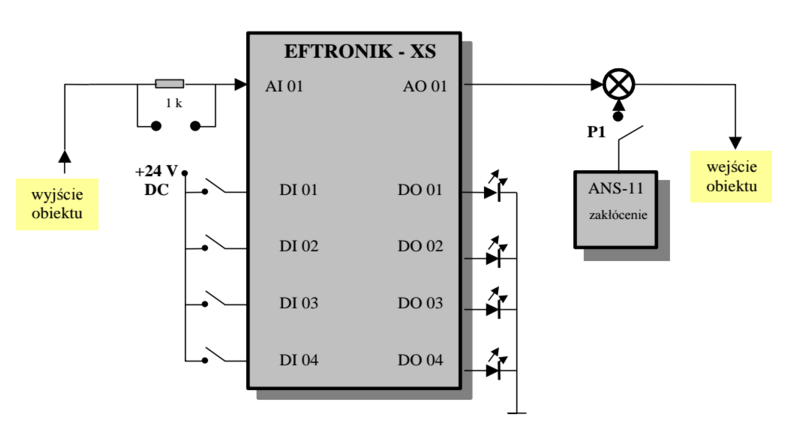
\includegraphics[width=0.75\textwidth]{./img/stanowisko.png}
		\end{figure}
		Eftronik XS jest przemysłowym regulatorem cyfrowym, wyposażonym w funkcję samostrojenia, używanym przez nas w ćwiczeniu do realizacji algorytmu PID wraz z dobraniem jego parametrów. Regulator ten obsługujemy poprzez panel użytkownika, poruszając się pomiędzy warstwami odpowiadającymi za grupy funkcji regulatora. Oprócz tego mamy do dyspozycji oscyloskop z możliwością pobrania danych na nośnik USB oraz termiczny obiekt regulacji.
	\section{Obiekt regulacji}
		Jest to obiekt cieplny, którego sygnał wejściowy i wyjściowy jest sygnałem znormalizowanym z zakresu 0--5[mA]. Obiekt jest metalowym prętem wykonanym z miedzi, o długości 260 milimetrów, umieszczonym w obudowie zapewniającej izolację termiczną od otoczenia. Sterowanie na obiekcie jest realizowane przy pomocy elementu grzejnego umieszczonego na jednym z jego końców. Temperatura pręta jest mierzona termometrami rezystancyjnymi nawiniętymi w punktach 0,3, 0,5, 0,7 oraz 0,9 długości pręta.
		\begin{figure}[H]
			\centering
			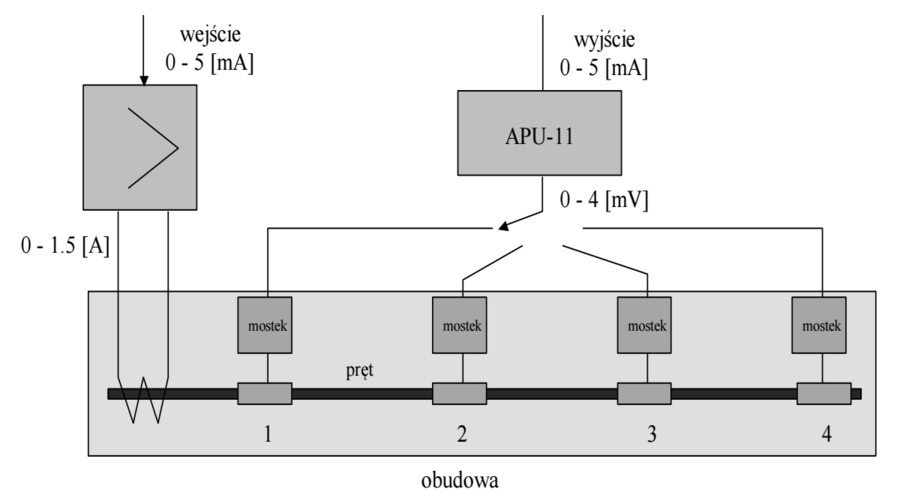
\includegraphics[width=0.75\textwidth]{./img/obiekt.png}
		\end{figure}
		Taka realizacja obiektu sterowania pozwala na ustawianie różnych stałych czasowych i opóźnień. Obiekt zachowuje się niesymetrycznie - inaczej się chłodzi niż nagrzewa.
	\section{Wykonanie ćwiczenia}
		Ćwiczenie rozpoczęliśmy od sprawdzenia, czy stanowisko działa poprawnie - zgraliśmy próbne dane z oscyloskopu, które przedstawiały stan ustalony, uzyskany przez poprzednią grupę.
		\begin{figure}[H]
			\centering
			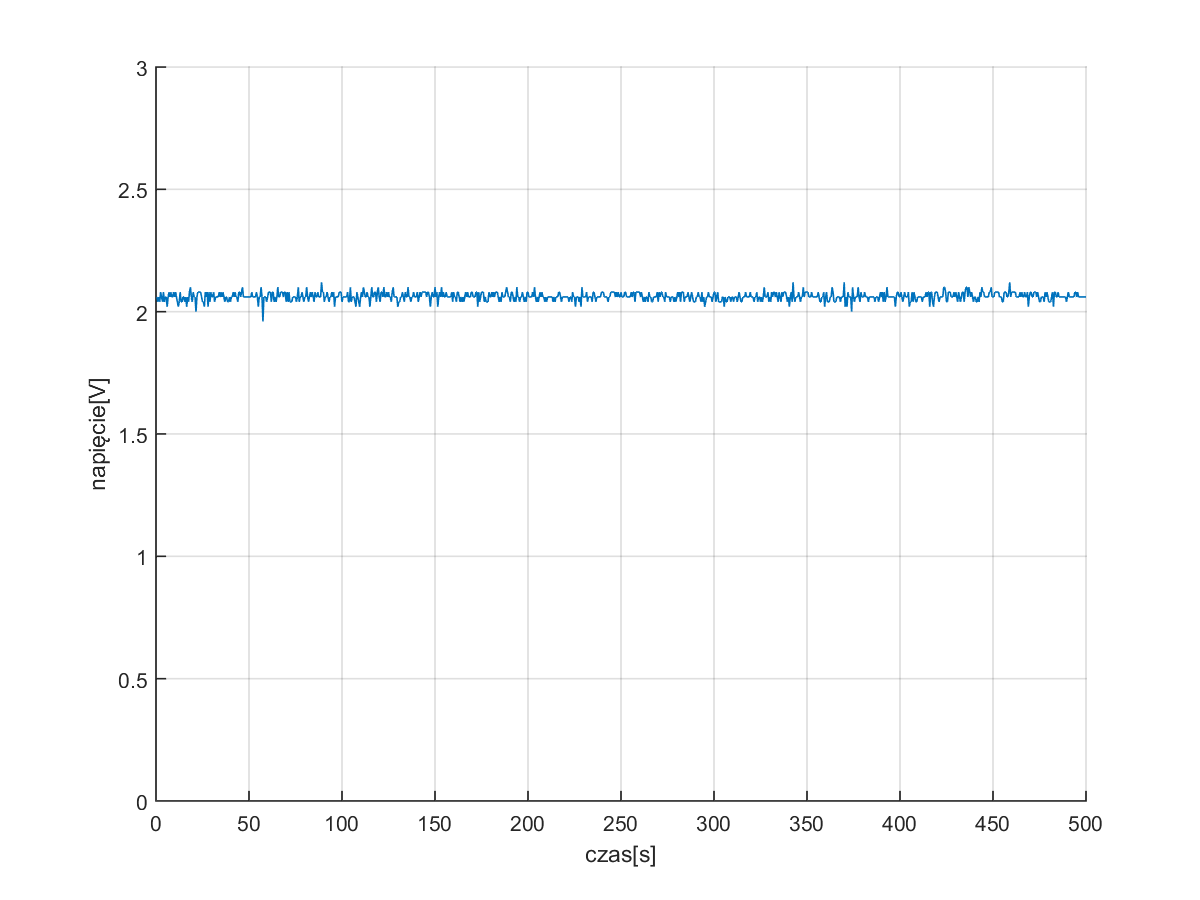
\includegraphics[width=0.75\textwidth]{./img/nothing.png}
		\end{figure}
		Można zauważyć, że dane z oscyloskopu znajdują się nieco powyżej stanu wskazywanego przez szafę. Widoczne na przebiegu są również pokaźne szumy, które jednak nie powinny wpływać na przebieg ćwiczenia.
		\subsection{Metoda Zieglera-Nicholsa}
			Strojenie metodą Zieglera-Nicholsa rozpoczęliśmy od wyzerowania czasu różniczkowania i wyłączenia czasu całkowania (wyzerowanie odpowiednich komórek). Potem zadaliśmy na wejście skok zaburzający, aby wyprowadzić układ ze stanu równowagi (około 30 sekund). Następnie przystąpiliśmy do szukania wartości wzmocnienia krytycznego.
			\subsubsection{$k_p = 2,4$}
				Na przebiegu poniżej można zauważyć, że amplituda gaśnie. Oznacza to, że wartość $k_p = 2,4$ jest za mała aby być wartością krytyczną wzmocnienia.
				\begin{figure}[H]
					\centering\
					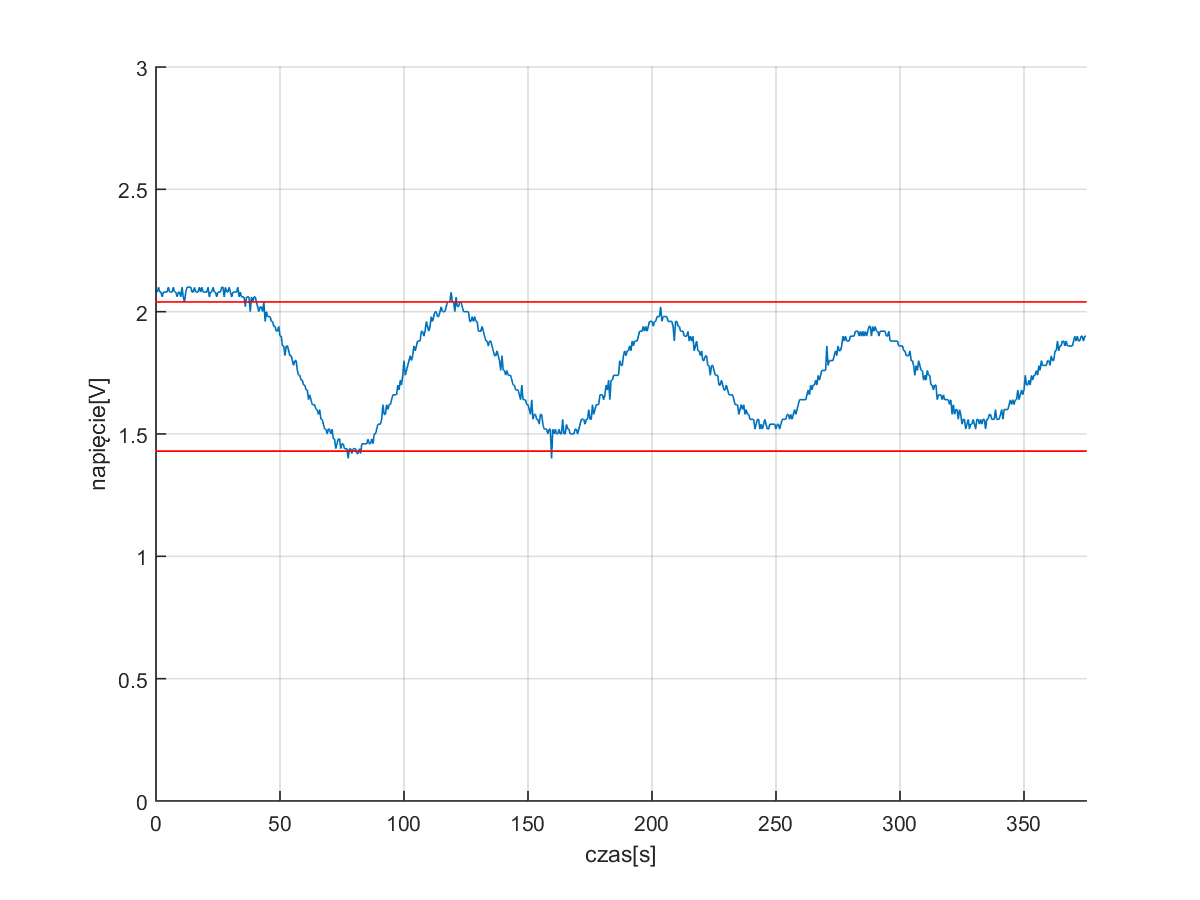
\includegraphics[width=0.75\textwidth]{./img/too_low.png}
				\end{figure}
			\subsubsection{$k_p = 2,9$}
				Na przebiegu poniżej można zauważyć, że amplituda rośnie. Oznacza to, że wartość $k_p = 2,9$ jest zbyt wysoka aby być wartością krytyczną wzmocnienia.
				\begin{figure}[H]
					\centering
					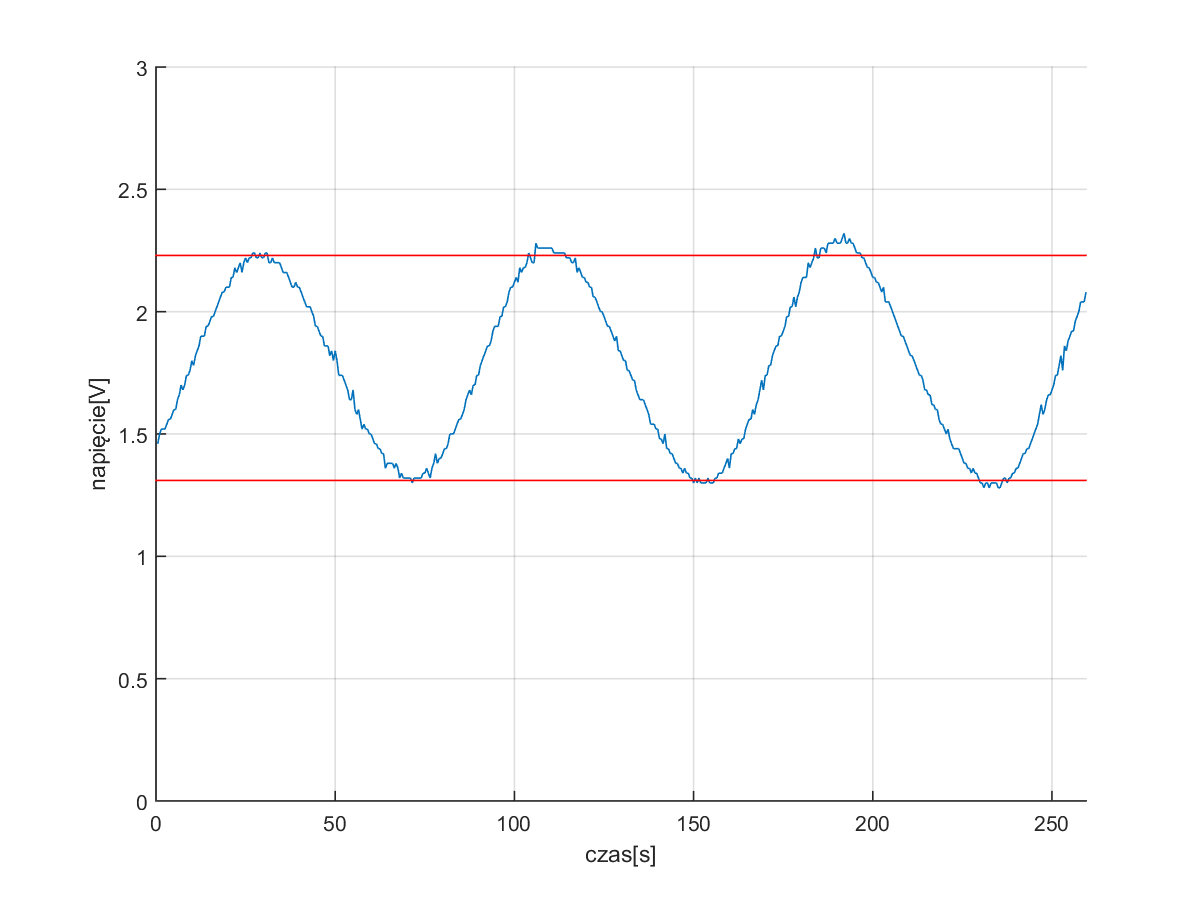
\includegraphics[width=0.75\textwidth]{./img/too_high.png}
				\end{figure}
			\newpage
			\subsubsection{$k_p = 2,7$}
				Oscylacje dla wzmocnienia $k_p$ = 2,7 okazują się być stałe. Jest to więc wzmocnienie krytyczne. Okres oscylacji jest zaznaczony na przebiegu jako interwał czasowy między największymi wartościami sygnału i wynosi $T_{osc} = 82$ s
				\begin{figure}[H]
					\centering
					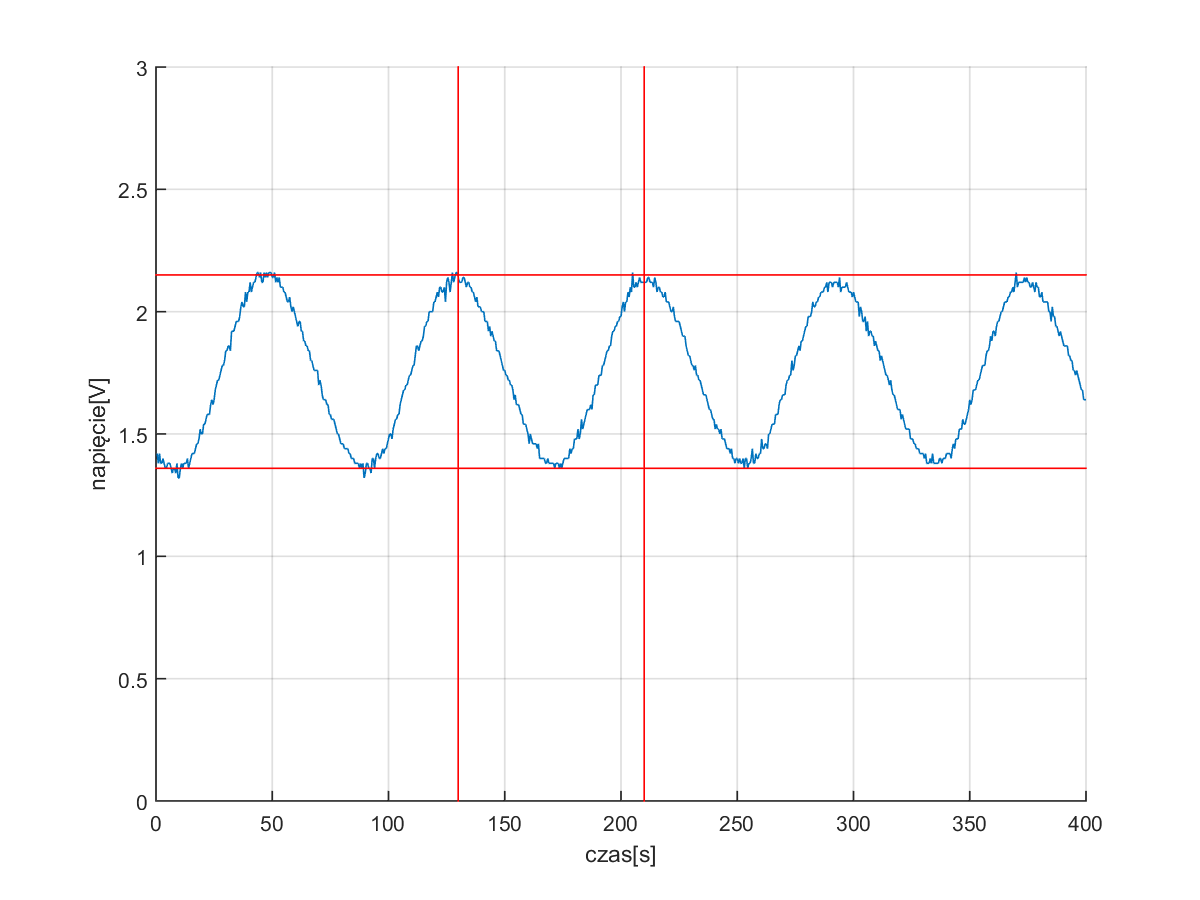
\includegraphics[width=0.75\textwidth]{./img/oki.png}
				\end{figure}
				Na podstawie tego jesteśmy w stanie wyznaczyć wszystkie parametry algorytmu PID ISA:
				\begin{itemize}
					\item $k_{p} = 0,6 \cdot k_{kr} =  1,62$ 
					\item $T_i = 0,5 \cdot T_{osc} = 41$
					\item $T_d = 0.125 \cdot T_{osc} = 10,25$
				\end{itemize}
				\begin{figure}[H]
					\centering
					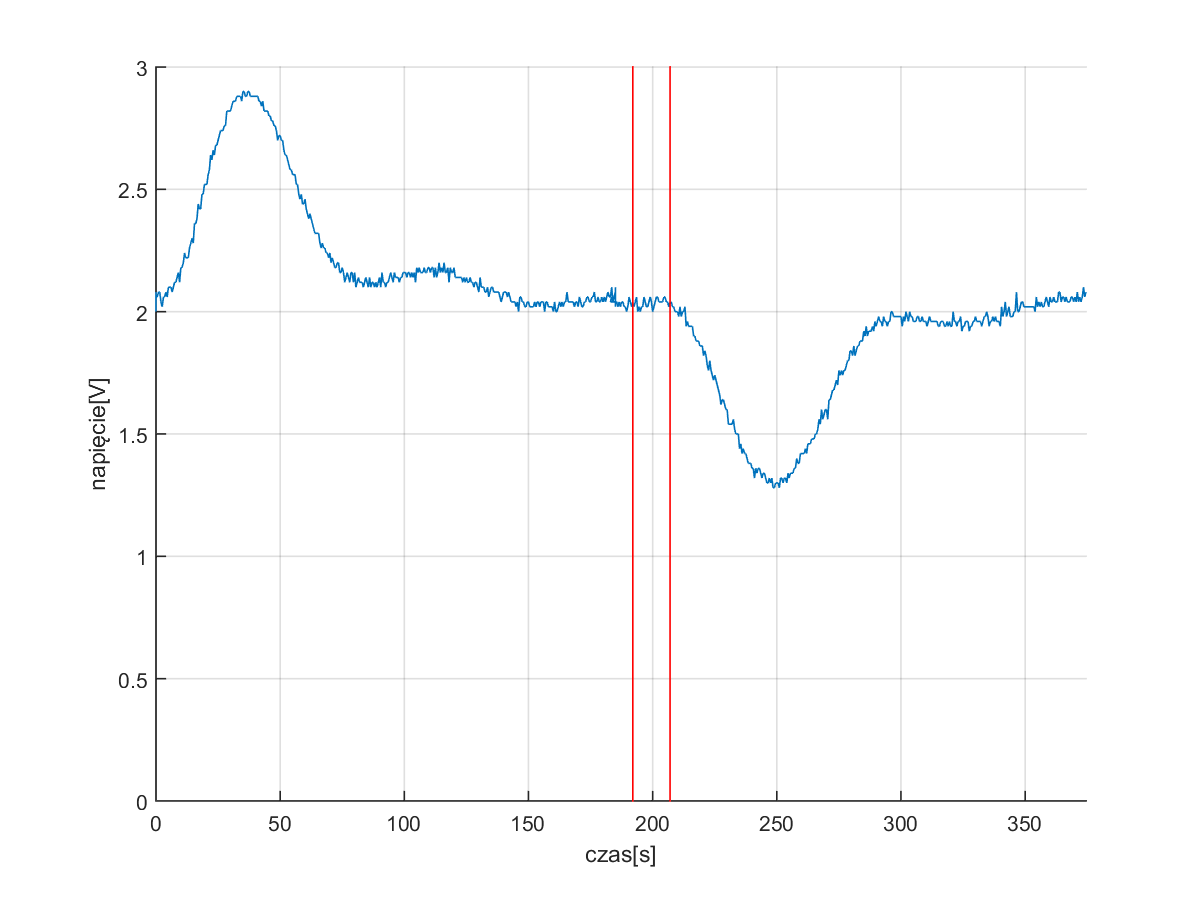
\includegraphics[width=0.75\textwidth]{./img/ZN.png}
				\end{figure}
				Przebieg ten przedstawia reakcję obiektu na zadane sterowanie z dostrojonego algorytmu PID metodą Zieglera-Nicholsa. Pionowe linie przedstawiają czas martwy - czas jaki musiał upłynąć od zadania przez nas zakłócenia na obiekt do chwili uzyskania od niego odpowiedzi. Zakłócenie zostało podane z początku przebiegu, a następnie po jego ustabilizowaniu się w chwili będącej wygodną do odczytu z oscyloskopu, zaprzestaliśmy podawać zaburzenie, co jest zauważalne drugim wybrzuszeniem na przebiegu. Z odczytu z pomiarów wnioskujemy, że czas martwy $\tau = 15 \ \mathrm{s}$.
		\subsection{Samostrojenie}
			Samostrojenie wykorzystuje metodę Astroma--Hagglunda. Proces strojenia składa się z łącznie trzech faz:
			\begin{itemize}
				\item[I] -- doprowadzenie układu do stanu równowagi
				\item[II] -- pomiar poziomu zakłóceń
				\item[III] -- właściwy eksperyment -- wprowadzenie układu w stan oscylacji o stałej amplitudzie przy pomocy regulatora dwupołożeniowego
			\end{itemize}
			\begin{figure}[H]
				\centering
				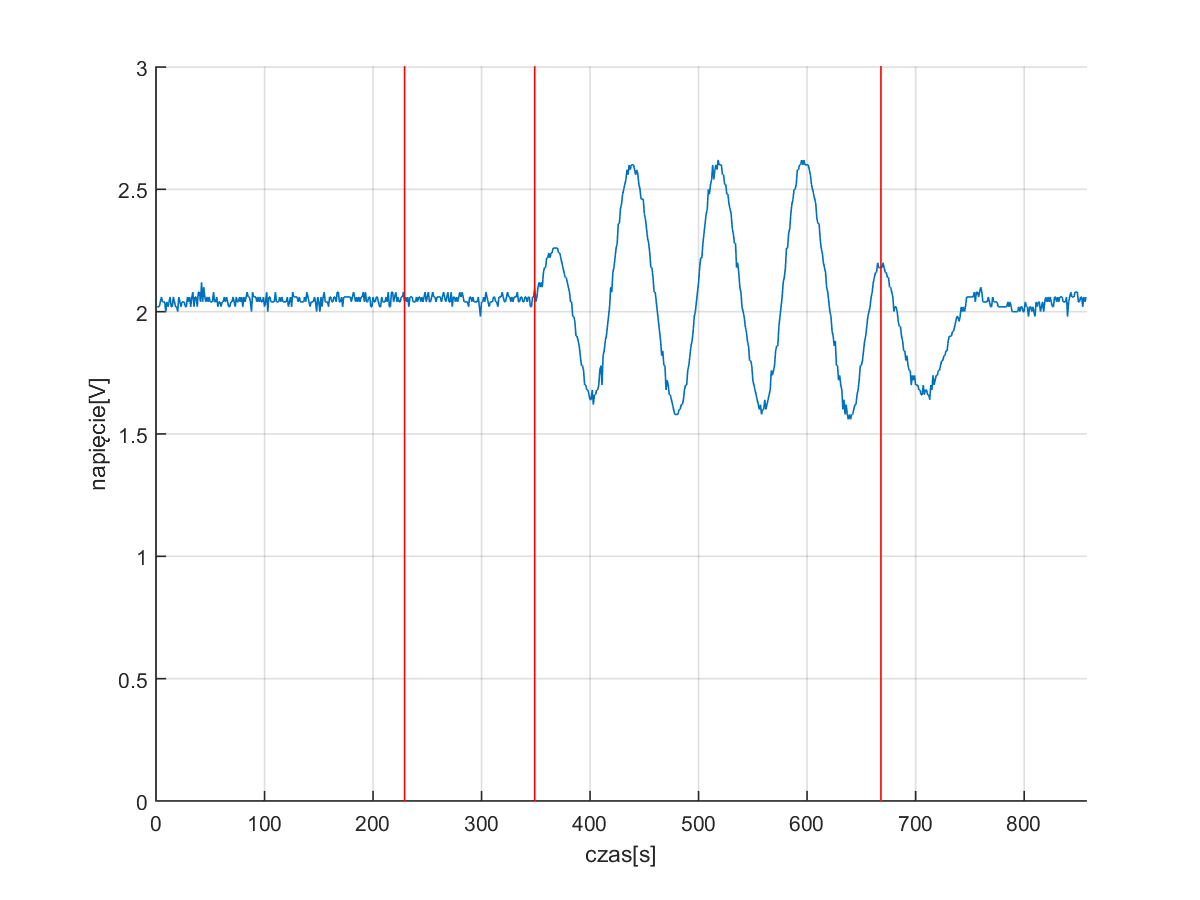
\includegraphics[width=0.75\textwidth]{./img/strojenie.png}
			\end{figure}
			Powyższy przebieg przedstawia proces samostrojenia z wydzielonymi fazami. Każda pionowa linia informuje o zakończeniu się kolejnej fazy. Parametry uzyskane w skutek przeprowadzenia samostrojenia:
			\begin{itemize}
				\item $k_{p} = 1,486$ 
				\item $T_i = 39$
				\item $T_d = 9,324$
			\end{itemize}
			Dla podanych parametrów przeprowadziliśmy te same doświadczenie, co przeprowadziliśmy dla strojenia metodą Zieglera-Nicholsa. Najpierw podaliśmy zaburzenie, następnie poczekaliśmy aż sygnał się ustabilizuje i stan będzie łatwy do odczytania na oscyloskopie, a następnie przestaliśmy podawać zaburzenie. \newpage
			Na pierwszy rzut oka można zauważyć, że mamy do czynienia z podobnym przebiegiem jak w przypadku nastawień uzyskanych z poprzedniego strojenia. Podobnie jak tam zarejestrowaliśmy ten sam czas martwy, który wynosi $\tau = 15\ \mathrm{s}$
			\begin{figure}[H]
				\centering
				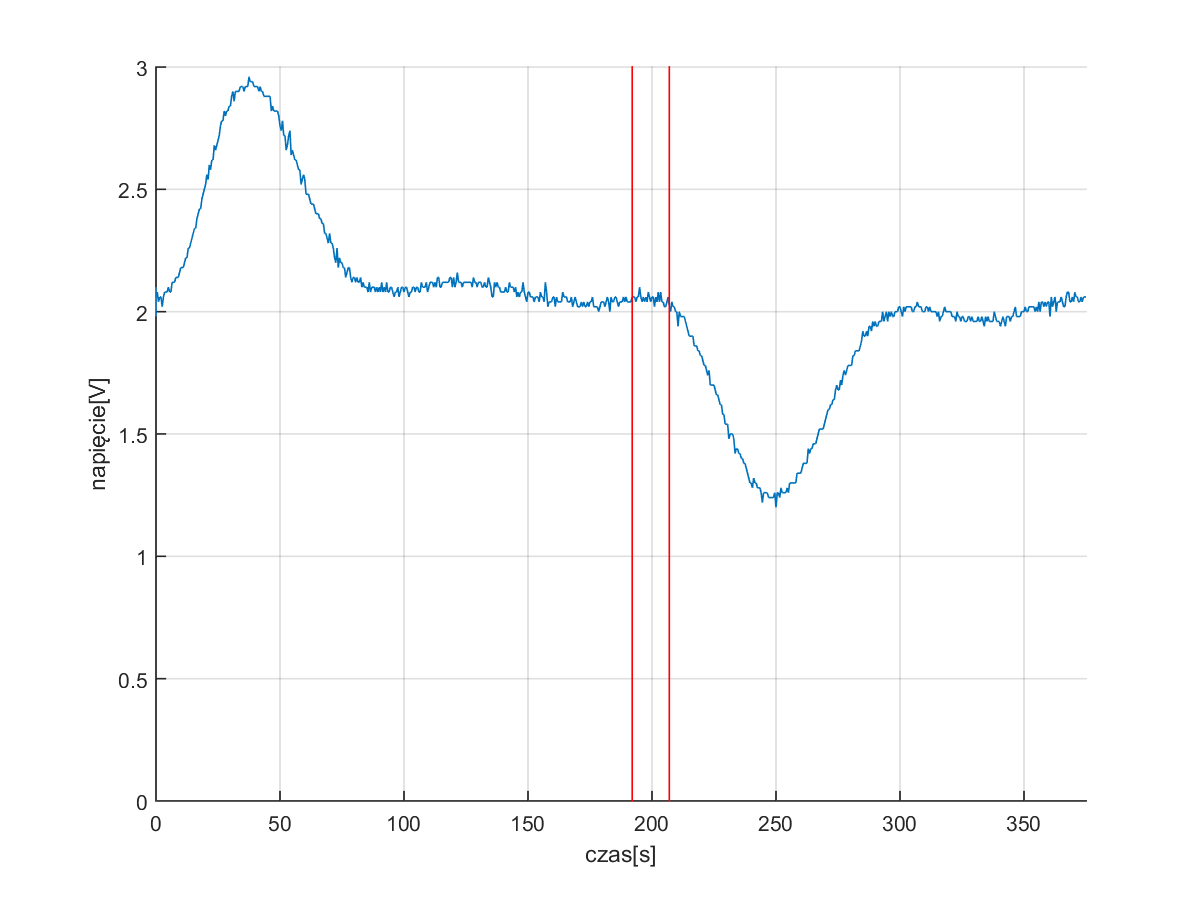
\includegraphics[width=0.75\textwidth]{./img/auto.png}
			\end{figure}
		\subsection{Porównanie metod}
			Po nałożeniu obydwu przebiegów na siebie można zobaczyć, że zachowują się niemalże identycznie, jednak przy parametrach uzyskanych z automatycznego strojenia dochodzi do większych wartości uchybu.
			\begin{figure}[H]
				\centering
				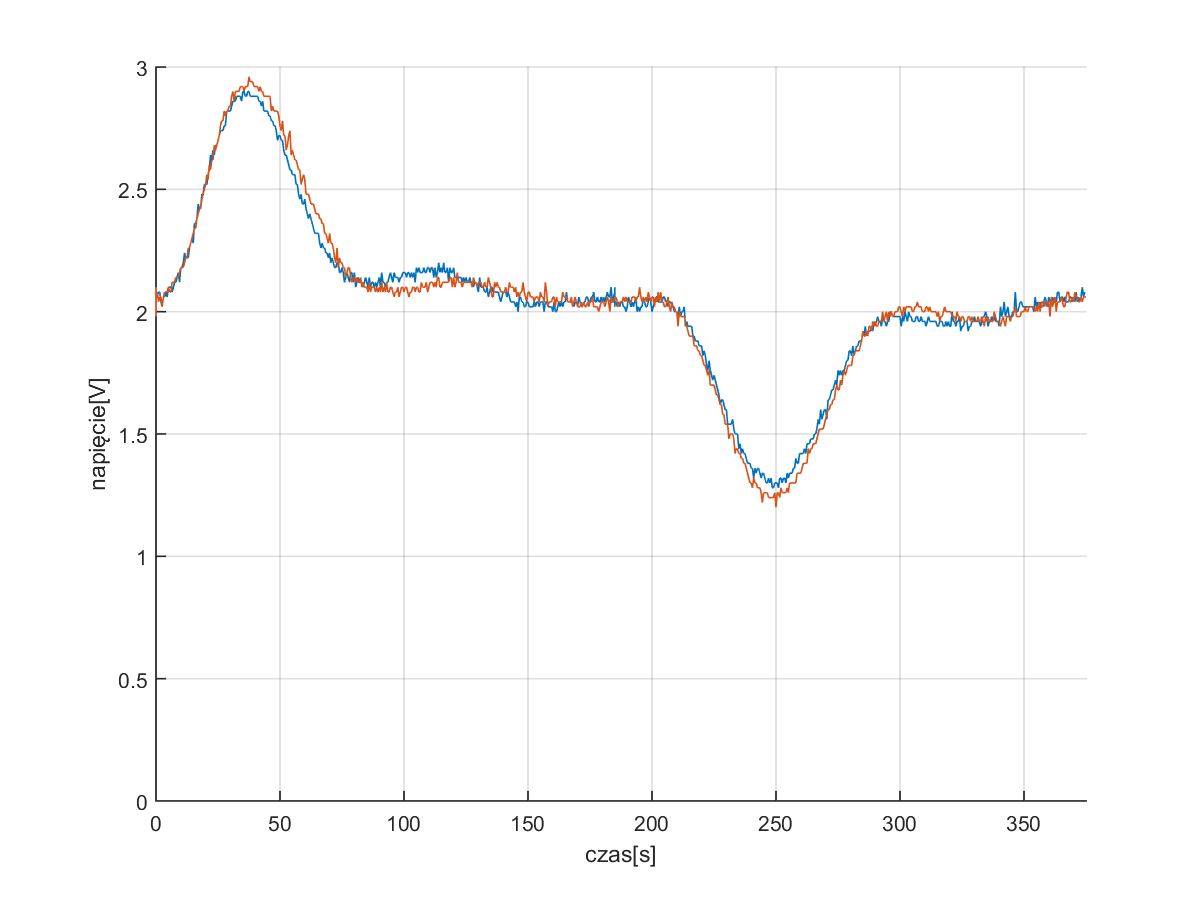
\includegraphics[width=0.75\textwidth]{./img/comparision.png}
			\end{figure}
			Można stwierdzić, że metoda Zieglera-Nicholsa jest efektywniejsza w doborze parametrów i algorytm PID dla parametrów przez nią dobranych ma mniejsze przesterowania (przy samostrojeniu pierwsze maksimum jest większe nisz w metodzie Zieglera-Nicholsa, a drugie jest mniejsze). Oprócz tego zastosowaliśmy całkowy wskaźnik jakości jakim jest:
			$$
				J = \int_{0}^{+\infty} e^2(t) \mathrm{d}t
			$$
			Ograniczyliśmy się jednak do skończonego przedziału czasu, a ze względu na dużą liczbę punktów pomiarowych wykorzystaliśmy metodę trapezów do przybliżenia całki. Współczynnik ten wyniósł u nas dla metody Zieglera--Nicholsa $J_{ZN} = 20,88$, a dla samostrojenia $J_s = 23,98$. Jest to wynik zgodny z przewidywaniami teoretycznymi, gdyż metoda Zieglera--Nicholsa powinna dawać wynik optymalny biorąc pod uwagę całkę z kwadratu błędu. Ze względu na niesymetryczność zachowania się układu w trakcie ogrzewania i chłodzenia uśredniliśmy wyniki z reakcji na zadanie i zabranie zakłócenia.
		\section{Wnioski}
			Najważniejszym wnioskiem, który nasunął się nam na myśl w trakcie opracowywania wyników było to dlaczego w czasie poszukiwania wartości krytycznej wzmocnienia sygnał nie oscylował wokół wartości ustalonej, tylko wokół wartości od niej niższej. Wzięło się to stąd, że regulator typu P posiada uchyb ustalony, który bardzo często jest trudny do zaobserwowania ze względu na bardzo duże wartości wzmocnienia. Tu jednak mieliśmy do czynienia z wartościami stosunkowo małymi, rzędu jedności, co pozwoliło nam na obserwację uchybu ustalonego. Dokonaliśmy tego w sposób pośredni dzięki obserwacji wyjścia.
			\newline
			\newline
			W trakcie dokonywania obliczeń doszliśmy do tego, że mimo podobnych wyników, metoda Zieglera-Nicholsa jest lepsza pod względem zastosowanego przez nas kryterium całkowego oraz przesterowań. Sprawdziliśmy tym samym, czy naprawdę osiągnie lepszy wynik w kryterium, które zgodnie z teorią optymalizuje, uzyskując wynik pozytywny. 
			\newline
			\newline
			W trakcie przeprowadzenia ćwiczenia zaobserwowaliśmy negatywny wpływ opóźnień w układzie na sterowanie nim. Były to wartości bliskie 50\% wartości ustalonej, przez co mogłyby doprowadzić do błędnego przebiegu procesu sterowania. Doprowadziły one do oscylacji, a w skrajnym przypadku nawet do utraty stabilności układu.
			\newline 
			\newline
			Jednak mimo wielu zalet obydwu metod strojenia, takich jak brak konieczności posiadania wiedzy na temat obiektu sterowania mogliśmy zaobserwować ich dwie wielkie wady. Strojenie tymi metodami trwa bardzo długo oraz prowadzi często do przekroczenia wartości zadanej. Takie zachowanie może być niedopuszczalne, jeżeli mamy do czynienia z układem o bardzo dużej stałej czasowej i czasie martwym takim jak chociażby piec hutniczy lub z niebezpiecznymi substancjami, dla których nawet nieznaczne przekroczenie wartości zadanej może oznaczać wybuch.
			\newline
			\newline
			
\end{document}